% Chapter 4
\chapter{Conception}

\label{Chapter4} 
le Software-Defined Networking a rapidement émergé comme une technologie prometteuse pour les réseaux futurs et a gagné beaucoup d'attention. Cependant, la nature centralisée du SDN rend le système vulnérable aux attaques par déni de service (Dos), une fois le contrôleur compris, tout le réseau cessera de fonctionner. Mais cette centralisation a un avantage, la gestion centralisée des équipements réseau, elle permet d'avoir une vue globale des flux de trafic, ce qui offre un meilleur système de défense contre les attaques DoS.\\

Comme mentionné dans la section \ref{rDoS}, nous nous intéressons dans notre travail à une attaque DOS spécifique, connue sous le nom de \textbf{Reflective-DoS} (RDos). Cette attaque est un peu spéciale et diffère carrément des autres types d'attaques Dos, dans le principe de fonctionnement et les dommages causés. On parlera plus sur cette attaque dans la section suivante. \\

Ce chapitre portera sur la conception de notre solution. Nous commençons par la problématique et la motivation de notre travail, suivi des hypothèses de conception. On passera après à la première étape de la conception, où on présentera l'architecture de notre système et ses différents composants. L'étape suivante est la construction de notre modèle de clustering  et terminera évidemment avec une conclusion sur le travail effectué.

\section{Problématique}
Mars 2018, un nouveau record a été marqué avec 1.7 Tbps de trafic généré par une attaque DoS réflective. La compagnie \textbf{Arbor Networks} a affirmé que son système d'analyse de trafic, ATLAS, a enregistré 1.7 Tbps d'une attaque reflective contre un site web d'un client[\cite{19}].\\

RDoS n’attaque pas directement la cible mais envoie plutôt plusieurs requêtes vers un service tiers exploitable (c. -à-d. le réflecteur, généralement c'est un serveur) avec une adresse IP d’expéditeur usurpée, ce qui rend l'attaquant anonymat. Les réponses du serveur tiers sont ensuite envoyées à la cible d’attaque réelle et causer une surcharge. Les protocoles avec des messages de réponse qui sont beaucoup plus grands que les messages de demande sont particulièrement bien adapté à ces attaques en raison des effets d’amplification. La nature de ces attaques nécessite des services qui fonctionnent sans connexion établie entre le client et le serveur. Une étude récente[\cite{20}] a trouvé que $ 99.72\% $ des attauqes RDoS utilisent des protocols basé UDP, comme DNS, NTP, ..etc. Les messages reçus dans une attaque RDoS sont difficiles à différencier du trafic bénin, car ils sont conformes aux spécifications du protocole. Les réflecteurs sont correctement gèrent toutes les demandes comme légitimes, mais l’absence de réponse est une caractéristique des attaques réflectives qui ne peut être masquée.

\begin{figure}[h]
\centering
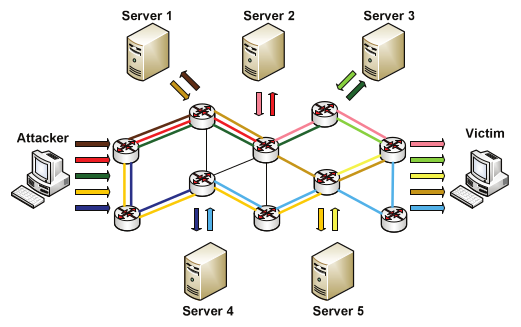
\includegraphics[width=0.7\textwidth]{Figures/rDoS}
\decoRule
\caption{Principe de dénie de service réflectif}
\label{fig:rDoS}
\end{figure} 

À ce niveau, on peut clairement voir que l'impact de ce type d'attaque est en double; en premier lieu, la consommation de la bande passante des liens réseau à cause au nombre excessive des messages requêtes et réponses échangés. En deuxième lieu, la surchage des serveurs tiers avec des messages requêtes, qui vont les traiter évidemment, car pour eux ils paraissent des requêtes légitimes.\\ 

\section{Motivation du travail}
Un article[\cite{21}] sur les travaux connexes a montré que la défense contre les attaques RDoS peut être divisée en 3 principales tâches : (1) surveillance (\textit{monitoring}) et la collecte de données du trafic réseau, (2) l’interprétation de ces données et la détection d’une attaque en cours, et (3) la mitigation de l’attaque. Selon leurs tâches principales, les solutions existantes varient considérablement dans leurs hypothèses et leurs exigences.\\
Dans la littérature on trouve que la surveillance du trafic, qui représente la première phase du processus de détection, se fait sur ces trois couches:\\
\begin{itemize}
\item[•] La couche réseau.
\item[•] La couche de transport.
\item[•] La couche d'application.\\
\end{itemize}

Par exemple \textit{PacketScore}, par Kim et al [\cite{22}], utilise le statistiques de paquets collectés pour comparer chaque paquet reçu au trafic bénin et d’attaque pour ensuite lui attribuer une note. Les paquets qui sont similaires au trafic d’attaque sont éliminés. Cette approche nécessite une surveillance active de la couche réseau.
Plusieurs autre travaux, [\cite{23}, \cite{24}] s'interèsse à la couche de trasnport pour la détection des anomalies en analysant les paquets de transport, ICMP, TCP et UDP.\\

Pour cette fin, nous proposons une solution, basée sur une approche de clustering, pour la détéction des d'attaque DoS réflectives dans un réseau SDN. Cette solution prend en charge aussi les attaques DoS du type UDP-Flooding (voir section \ref{rDoS}). La mitigation de l'attaque ne fait par partie de notre travail, on ferra juste la détection. La première tâche, surveillance te collecte de données, va être lancer sur la couche de transport, où on surveillera spécialement le protocole de transport UDP, vu qu'il est le plus utilisé dans les attaques RDoS. Pour la deuxième phase, qui est la détection, on utilisera notre modèle d'apprentissage pour analyser les données collectées dans la phase précédente et décider si c'est une attaque ou non.  

\section{Présentation de la Solution}
Les caractéristiques inhérentes des attaques de RDoS représentent un défis pour leur détection. Une surveillance et analyse continues du trafic réseau est nécessaire pour la détection des flux malins. La solution qu'on propose, pour ce fait, est un système de détection, appelé \textbf{F-DoS}, qui sera déployé dans le réseau cible pour assurer la surveillance du trafic au but de détecter des attaques DoS (RDoS et UDP-Flooding).\\

Ces deux fonctions de surveillance et de détection sont assurer par deux modules intégrée dans notre système. Le premier module, appelé \textbf{ARGUS}[28], est un annalyseur de flux, qu'on utilise pour capturer le trafic qui circulent dans le réseau, pour ensuite caculer les propriétés de chaque flux capturé. Les propriétés calculées vont être ensuite envoyées au deuxième module, appellé \textbf{FK-Means}. Ce dernier est un modèle de Clustering, qui prend en entrée les propriétés d'un flux et le met dans un des clusters préexistant, y'en a que deux clusters, un  pour le flux bénin et l'autre pour le flux malin (Attaques RDoS et UDP-Flooding).\\

L'architecture de notre système est illusté dans la figure suivante : \\


\section{Hypothèses}
Pour que notre système fonctionne de manière sûre et efficace, les hypothèses suivantes sont à prendre en considération :\\
\begin{itemize}
\item[•] Notre système est responsable de surveiller le réseau pour détecter uniquement les attaques de type DoS.\\
\item[•] On suppose que les liens entre le plan de données et le plan de contrôle sont fiables et dotés d’une bande passante suffisante pour faire circuler le trafic de contrôle nécessaire pour le fonctionnement du système et le protocole utilisé pour la communication entre ces deux plans est OpenFlow.\\
\item[•] Le réseau n’a pas été compromis avant ou durant le déploiement du système.\\
\item[•] Dernière hypothèse, qui est la plus importante. Notre modèle a été traîné sur le Dataset suivant xxxxxx. Tout résultat généré par ce système après son déploiement dépendra de cette Dataset.
\end{itemize}

 